\chapter{Analyse descendante}
    
	Nous avons réalisé l'analyse descendante de notre projet. 
	
	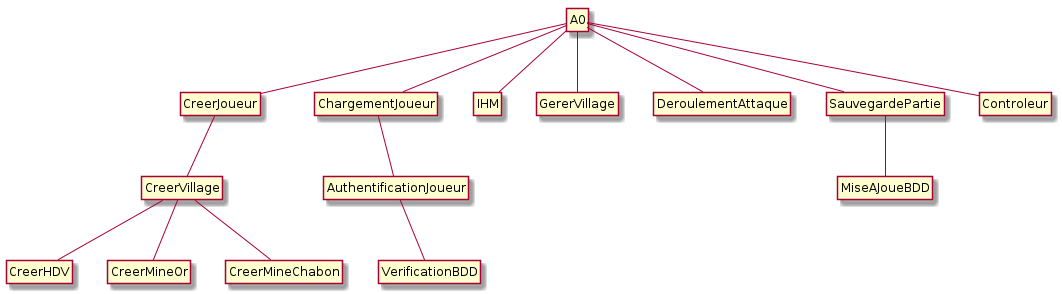
\includegraphics[scale=0.4]{graph/analyseDescendante.png}
	
	Ceci est la partie la plus générale de notre analyse descendante, on y voit les grands blocs : la gestion du village, l'IHM et le déroulement d'une attaque qui seront spécifiés ultérieurement. \\
	On distingue également la création du joueur, le controleur et la sauvegarde de la partie. 
	
	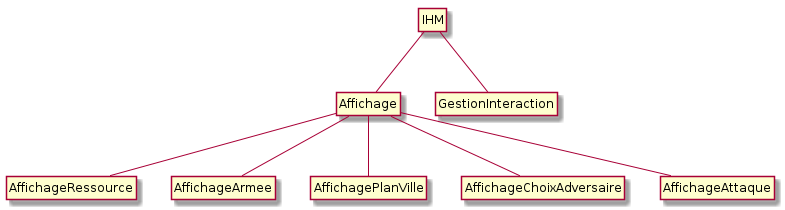
\includegraphics[scale=0.4]{graph/IHM.png}
	
	Pour l'IHM les grandes parties distinctes sont les interactions avec l'utilisateur (clavier, souris) ainsi que l'affichage des différentes parties : ressource, défense, ville etc

	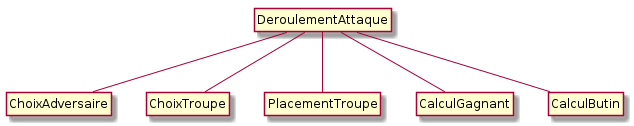
\includegraphics[scale=0.8]{graph/DeroulementAttaque.png}
	
	Pour le déroulement de l'attaque, on distingue comme parties importantes : le choix de l'adversaire, des troupes et le placement de nos unités par exemple. 

	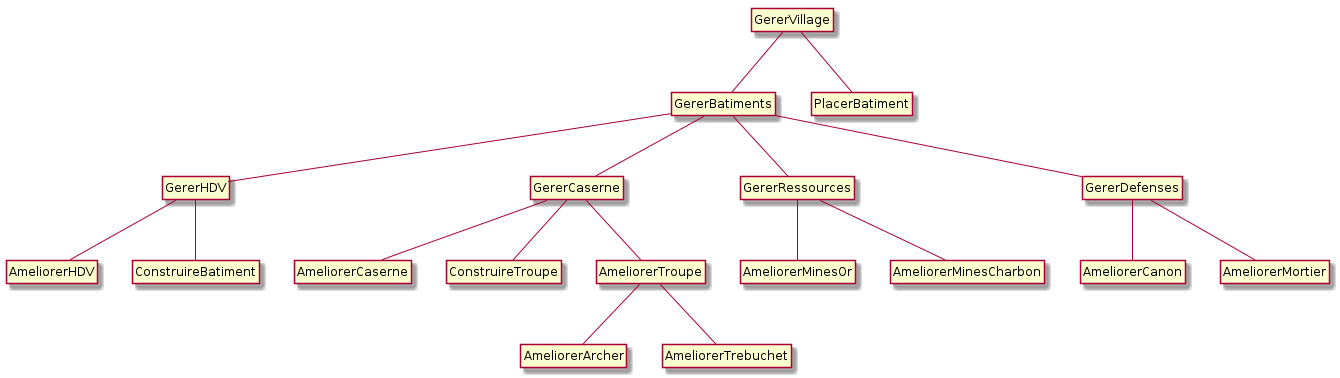
\includegraphics[scale=0.35]{graph/GestionVillage.png}
	
	Pour la gestion du village, il faut distinguer la gestion des bâtiments et de l'armée. Pour les bâtiments, on en distingue deux principaux : l'hôtel de ville (gestion de tous les bâtiments) et la caserne (gestion de toute l'armée). 

	
	